\documentclass[conference]{IEEEtran}
\IEEEoverridecommandlockouts
% The preceding line is only needed to identify funding in the first footnote. If that is unneeded, please comment it out.
\usepackage{cite}
\usepackage{amsmath,amssymb,amsfonts}
\usepackage{algorithmic}
\usepackage{graphicx}
\usepackage{textcomp}
\usepackage{xcolor}
\def\BibTeX{{\rm B\kern-.05em{\sc i\kern-.025em b}\kern-.08em
    T\kern-.1667em\lower.7ex\hbox{E}\kern-.125emX}}
\begin{document}

\title{Impact of Environment Topology on Robotic Swarm Aggregation: An Experimental Study with Atta-bots}

\author{
    \IEEEauthorblockN{
        Eduardo Fallas Valverde \IEEEauthorrefmark{1},
        Juan Carlos Brenes-Torres\IEEEauthorrefmark{1}, 
        Cindy Calderón-Arce\IEEEauthorrefmark{2}, 
        Rebeca Solís-Ortega\IEEEauthorrefmark{2}, \\
    }
    \IEEEauthorblockA{
        \IEEEauthorrefmark{1}Mechatronics Engineering School, Costa Rica Institute of Technology, Cartago, Costa Rica\\
        \IEEEauthorrefmark{2}Mathematics School, Costa Rica Institute of Technology, Cartago, Costa Rica\\
        Email: juanbrenes@tec.ac.cr
    }
}


\maketitle

\begin{abstract}
LO HACEMOS DE ULTIMO

\end{abstract}

\begin{IEEEkeywords}
component, formatting, style, styling, insert
\end{IEEEkeywords}

\section{Introduction}
CINDY 

Primer párrafo genérico sobre enjambres y el comportamiento de congregación. 

Referencias: Mencionar papers que hicieron experimentos de congregación y formation control. 

Mencionar que se trabaja mucho en la lógica/algortimo de como evadir obstáculos, ir en formación o congregarse, esto con la presencia de obstáculos y estos se prsentan en diferentes configuraciones. Pero se identifica un vacío en identificar como influye la cantidad de obstáculos, el tamaño y separación de estos en esos comportamientos.

Aporte: Caracterización experimental del impacto de la topología del entorno en el comportamiento de congregación de enjambres robóticos. 

\section{Materials and methods}

\subsection{Atta-bot robots}
The Atta-bot robotic platform is a differential-drive mobile robot designed as an agent for swarm research, in tasks such as exploration, collaborative navigation, and mapping in indoor environments (Figure \ref{fig:attas}). Its name is inspired by the Atta family of leaf cutter ants, which exhibit remarkable collective behaviors.
The first version of the robot was presented in \cite{Atta-Bot} and was successfully used for swarm experimentation in \cite{Brenes-Torres_2025, Adaptative-Brenes}.   This redesigned version, detailed in \cite{aguilera2024attabot}, substantially optimizes dimensions and mass compared to its predecessor, adopting a compact cylindrical chassis approximately 105 mm in diameter, and a rechargeable LiPo battery providing a continuous operating autonomy of more than 4 hours. 
Its electronic architecture unifies processing into a single ESP32 SoC microcontroller, which coordinates the actuators and integrated instrumentation, including wheel-coupled encoders for PID motion control, and a peripheral array of infrared proximity sensors for obstacle detection and avoidance. 
Finally, the robot communicates with the base station or other robots over a WiFi network using the UDP transport protocol, which minimizes transmission latency to allow a continuous stream of telemetry data, ensuring real-time swarm coordination.

\begin{figure}
    \centering
    \includegraphics[width=0.45\linewidth]{Atta_1_frente.jpg}
    \includegraphics[width=0.45\linewidth]{Atta_2_atras.jpg}
    \caption{Redesigned version of Atta-bot robot. Presents a compact design, enhanced maneuverability, WiFi communication, improved components and longer battery life.  }
    \label{fig:attas}
\end{figure}


\subsection{Robot tracking system}
EDUARDO

Explicar que el tracking de las posiciones y orientaciones del robot se hace mediante un sistema de visión por computadora cenital (techo) que usa tags Aruco.

\subsection{Robot behaviors}
EDUARDO

Explicar el comportamiento usado para evitar obstáculos. Explicar bien en detalle el comportamiento de congregación. Se pueden usar ecuaciones o pseudocódigo.
Poner fórmula para el radio de congreción.

\subsection{Swarm simulation}
EDUARDO

Explicar que se usó el simulador Webots, que se implementó un modelo físico de los attabos y lógico de sus comportamientos.
Que la intención es probar el enajmbre en un caso con escenario de mayores dimensiones y más robots, para ver la escalabilidad.

\subsection{Scenario topology and aggregation metrics}

The environment used for experimentation consisted on a (2,40 x 1,75) m flat surface with closed walls and obtacles placed at the middle (Figure \ref{fig:escenario}). Since the article seeks to indentify key elements on the scenario topology that  affects aggregation behavior, several obstacle configurations were defined by using two obstacle sizes and two gap widths between obstacles. 
Obstacles size were of approximate $0.74 \cdot a_{robot}$ (a=area), obstacle area less than the robot size, and $1.48 \cdot a_{robot}$, area larger than the robot size. The used passage gap width between obstacles were of $2 \cdot d_{robot}$ (d=diameter) and $4 \cdot d_{robot}$. The obstacles total area was between 1,2\% and 1,5\% of the total scenario area, this ratio was keep constant among the different configurations. 

Accordingly the validated configurations were: 
\begin{itemize}
    \item Scenario free of obstacles
    \item $0.74 \cdot a_{robot}$ obstacles and $2 \cdot d_{robot}$ gaps
    \item $0.74 \cdot a_{robot}$ obstacles and $4 \cdot d_{robot}$ gaps
    \item $2.12 \cdot a_{robot}$ obstacles and $2 \cdot d_{robot}$ gaps
    \item $2.12 \cdot a_{robot}$ obstacles and $4 \cdot d_{robot}$ gaps
\end{itemize}


\begin{figure}
    \centering
    \includegraphics[width=0.7\linewidth]{escenario.JPG} \\
    (a) \\ 
    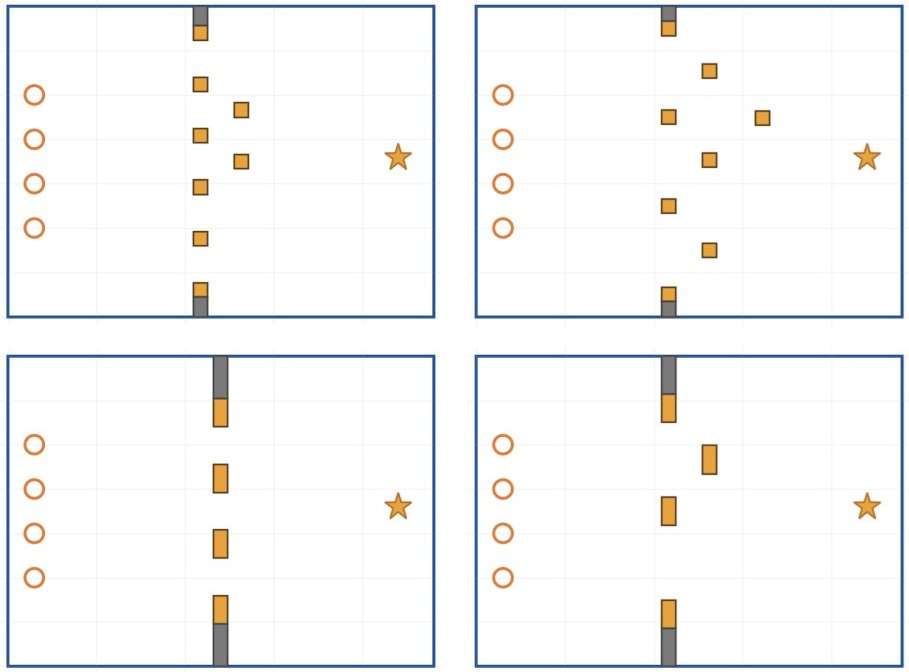
\includegraphics[width=0.95\linewidth]{scenario_configurations.jpg} \\
    (b)
    \caption{Experimental scenario configuration. (a) Controlled environment used for physical swarm validation. (b) Obstacles and gaps configurations.}
    \label{fig:escenario}
\end{figure}

In order to measure the impact of the scenario topology on the aggregation of the robot swarms, several metrics were used: 
\begin{itemize}

    \item Robot distance: accumulated distance traveled by each robot. Normalized by the euclidean distance from start point to final aggregation point.
    
    \item Aggregation time: defined from the start of the experiment and finalizes when the 90\% of agents reach the aggregation zone.
    
    \item Swarm compactness: measures how disperse is the swarm during each time of the experiment. Calculated by the squared root summatory of euclidean distances from each robot position to the swarm centroid, as defined in equation \ref{eq:compaction}, \ref{eq:centroid} and \ref{eq:avg_xy}. Values were normalized by the robot diameter.

\end{itemize}
 

\begin{equation}
    swarm_{comp} = \sqrt{\frac{1}{N} \sum_{i=1}^N \vert{} p_i(t) - p_{centroid}(t) \vert{}^2}
    \label{eq:compaction}
\end{equation}

\begin{equation}
    p_{centroid}(t)= (\bar{x}(t), \bar{y}(t)) 
    \label{eq:centroid}
\end{equation}

\begin{equation}
    \bar{x}(t) = \frac{1}{N}\sum_{i=1}^N x_i(t), \quad \bar{y}(t) = \frac{1}{N}\sum_{i=1}^N y_i(t)
    \label{eq:avg_xy}
\end{equation}


\section{Results and analysis}
TODOS

\begin{figure}
    \centering
    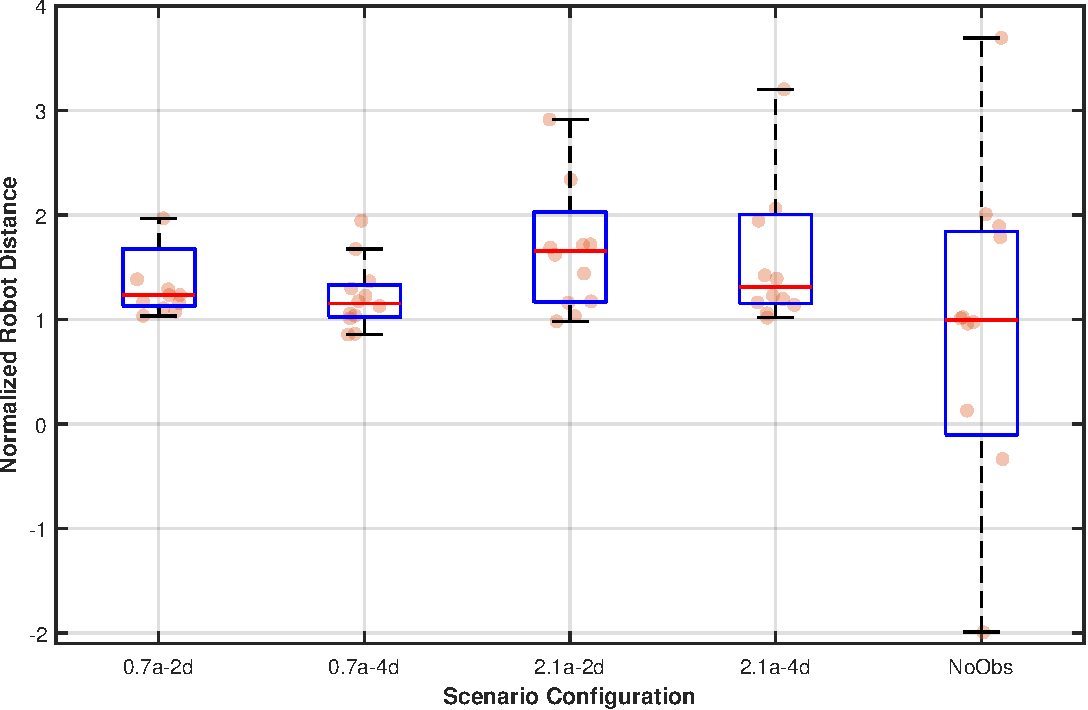
\includegraphics[width=0.8\linewidth]{Fig1_Normalized_Distance.pdf} \\
    (a) \\
    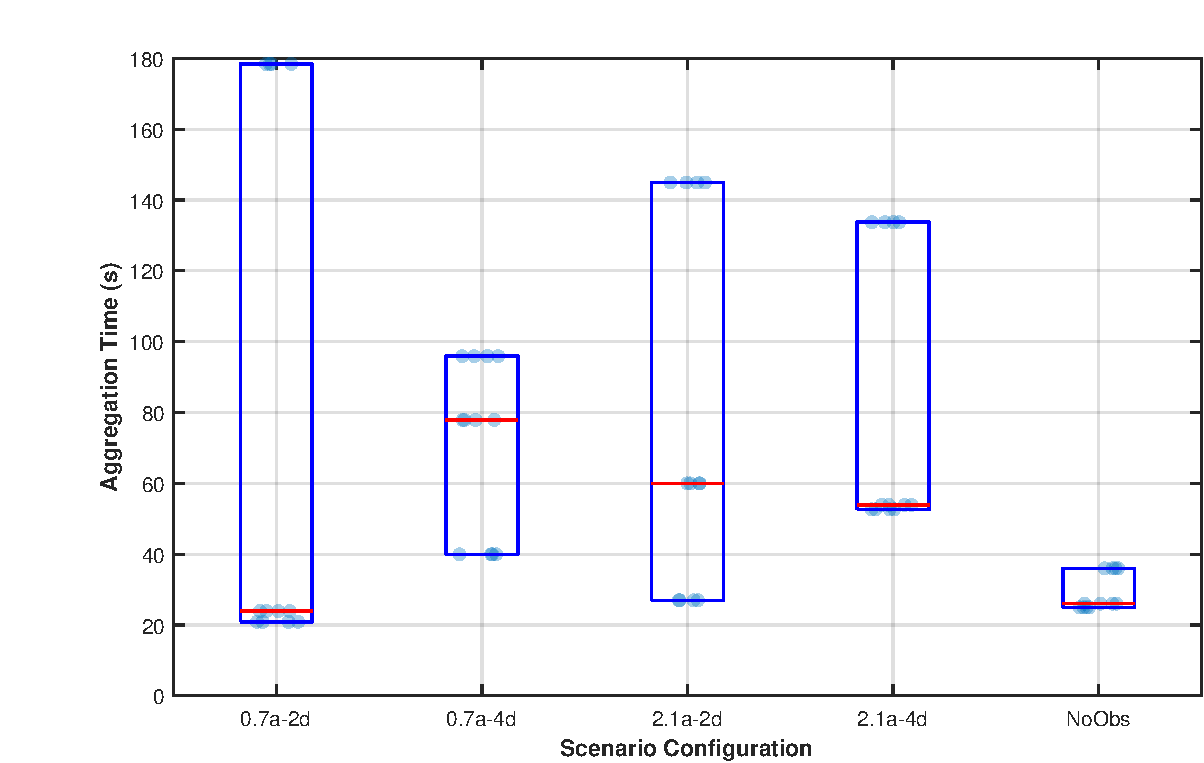
\includegraphics[width=0.8\linewidth, trim= 48 0 0 0, clip ]{Fig2_Aggregation_Time.pdf} \\
    (b) \\
    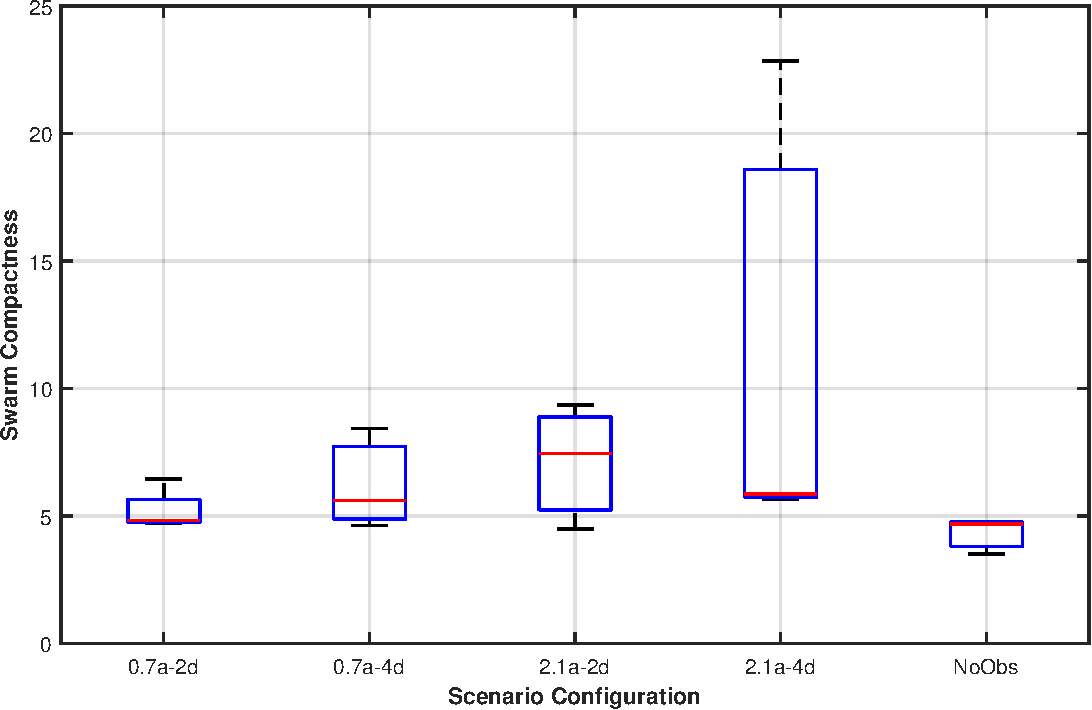
\includegraphics[width=0.8\linewidth]{Fig3_Final_Compactness.pdf} \\
    (c)
    \caption{Validation results with physical robot swarm. (a) Normalized distance traveled by robots on each scenario configuration. (b) Final aggregation time for the robot swarm. (c) Swarm Compactness metric during validations.}
    \label{fig:boxplots}
\end{figure}


\section{Conclusions and future work}
JUAN CARLOS Y CINDY

Mencionar los resultados obtenidos y como se comparan con otros trabajos.
Decir que sigue luego de esto.

\section*{Acknowledgment}

Citar algun proyecto del TEC




\bibliographystyle{IEEEtran}

\bibliography{referencias}


\end{document}
